\section*{Experiment 5}
% Using Queueing Theory it can be shown that the mean delay for a work conserving single server queueing system with Poisson process arrivals and a general service time distribution (i.e., an M/G/1 queue) is given by2 
% dM/G/1 = X + λX2 2(1 − ρ) (2) 
% where X is the mean service time (SERVICE TIME), ρ is the product of the mean arrival rate and the mean service time, i.e., ρ = λX, λ = ARRIVAL RATE, and X2 = σ2 X +  ̄X2 is the second moment of the service time3. Note that the total delay of a customer is the sum of its service time and its queueing delay. Therefore, the two terms in Equation 2 are the mean service time and the mean queueing delay incurred by the customers, respectively.
% When the service times are fixed (i.e., an M/D/1 queue, as in the supplied simulation), σX = 0, and therefore, the mean delay can be written as 4 dM/D/1 =  ̄X(2 − ρ) 2(1 − ρ) Compare the results that you plotted in Parts 2 and 4 to this analytic result.
If the mean delay can for an M/D/1 queue system can be written as
\begin{equation}
	\bar{d}_{M/D/1}=\frac{\bar{X}(2-\rho)}{2(1-\rho)}
	\label{eq:eq2}
\end{equation}
then we can plot Expression~\ref{eq:eq2} with $\bar{X}=10$ for Experiment 2 and  $\bar{X}=30$ for Experiment 4. The plot for Expression~\ref{eq:eq2} can be seen in Figure~\ref{fig:exp5}. This figure matches the results from our simulations in Experiments 2 and 4, which can be seen by comparing Figure~\ref{fig:exp4} and Figure~\ref{fig:exp5}.

% \begin{figure}[h]
% \centering
% \begin{tikzpicture}
% 	\begin{axis}[
% 		title = {Mean Delay vs. \texttt{ARRIVAL\_RATE}},
% 		%width = 0.98\textwidth,
% 		%height = 400,
% 		%xmin = 0, xmax = 0.1,
% 		%ymin = -1000000, ymax = 1100000,
% 		%ylabel = Mean Delay, xlabel = \texttt{ARRIVAL\_RATE},
% 		%xticklabel style={
% 		%/pgf/number format/fixed,
% 		%/pgf/number format/precision=3
% 		%},
% 		%scaled x ticks=false,
% 		%yticklabel style={
% 		%/pgf/number format/fixed,
% 		%/pgf/number format/precision=3
% 		%},
% 		%scaled y ticks=false,
% 		%legend pos=north east,
% 		% some code for adding points
% 		%nodes near coords={%
% 		%\footnotesize
% 		%$(\pgfmathprintnumber
% 		%{\pgfkeysvalueof{/data point/x}},
% 		%\pgfmathprintnumber
% 		%{\pgfkeysvalueof{/data point/y}})$%
% 		%},
% 	]
% 	\addplot {(2-(10*x)) / (2*(1-(10*x)))};
% 	%\label{plot:exp4exp2}
% 	%\addlegendentry{Experiment 2}
% 	%\addplot table [y=$mean_delay$, x=$arr_rate$]{../data/exp4.dat};
% 	%\label{plot:exp4exp4}
% 	%\addlegendentry{Experiment 4}
% 	\end{axis}
% \end{tikzpicture}
% \caption{Experiment 5: Mean Delay vs. Arrival Rate}
% \label{fig:exp5}
% \end{figure}

\begin{figure}[h]
    \centering
    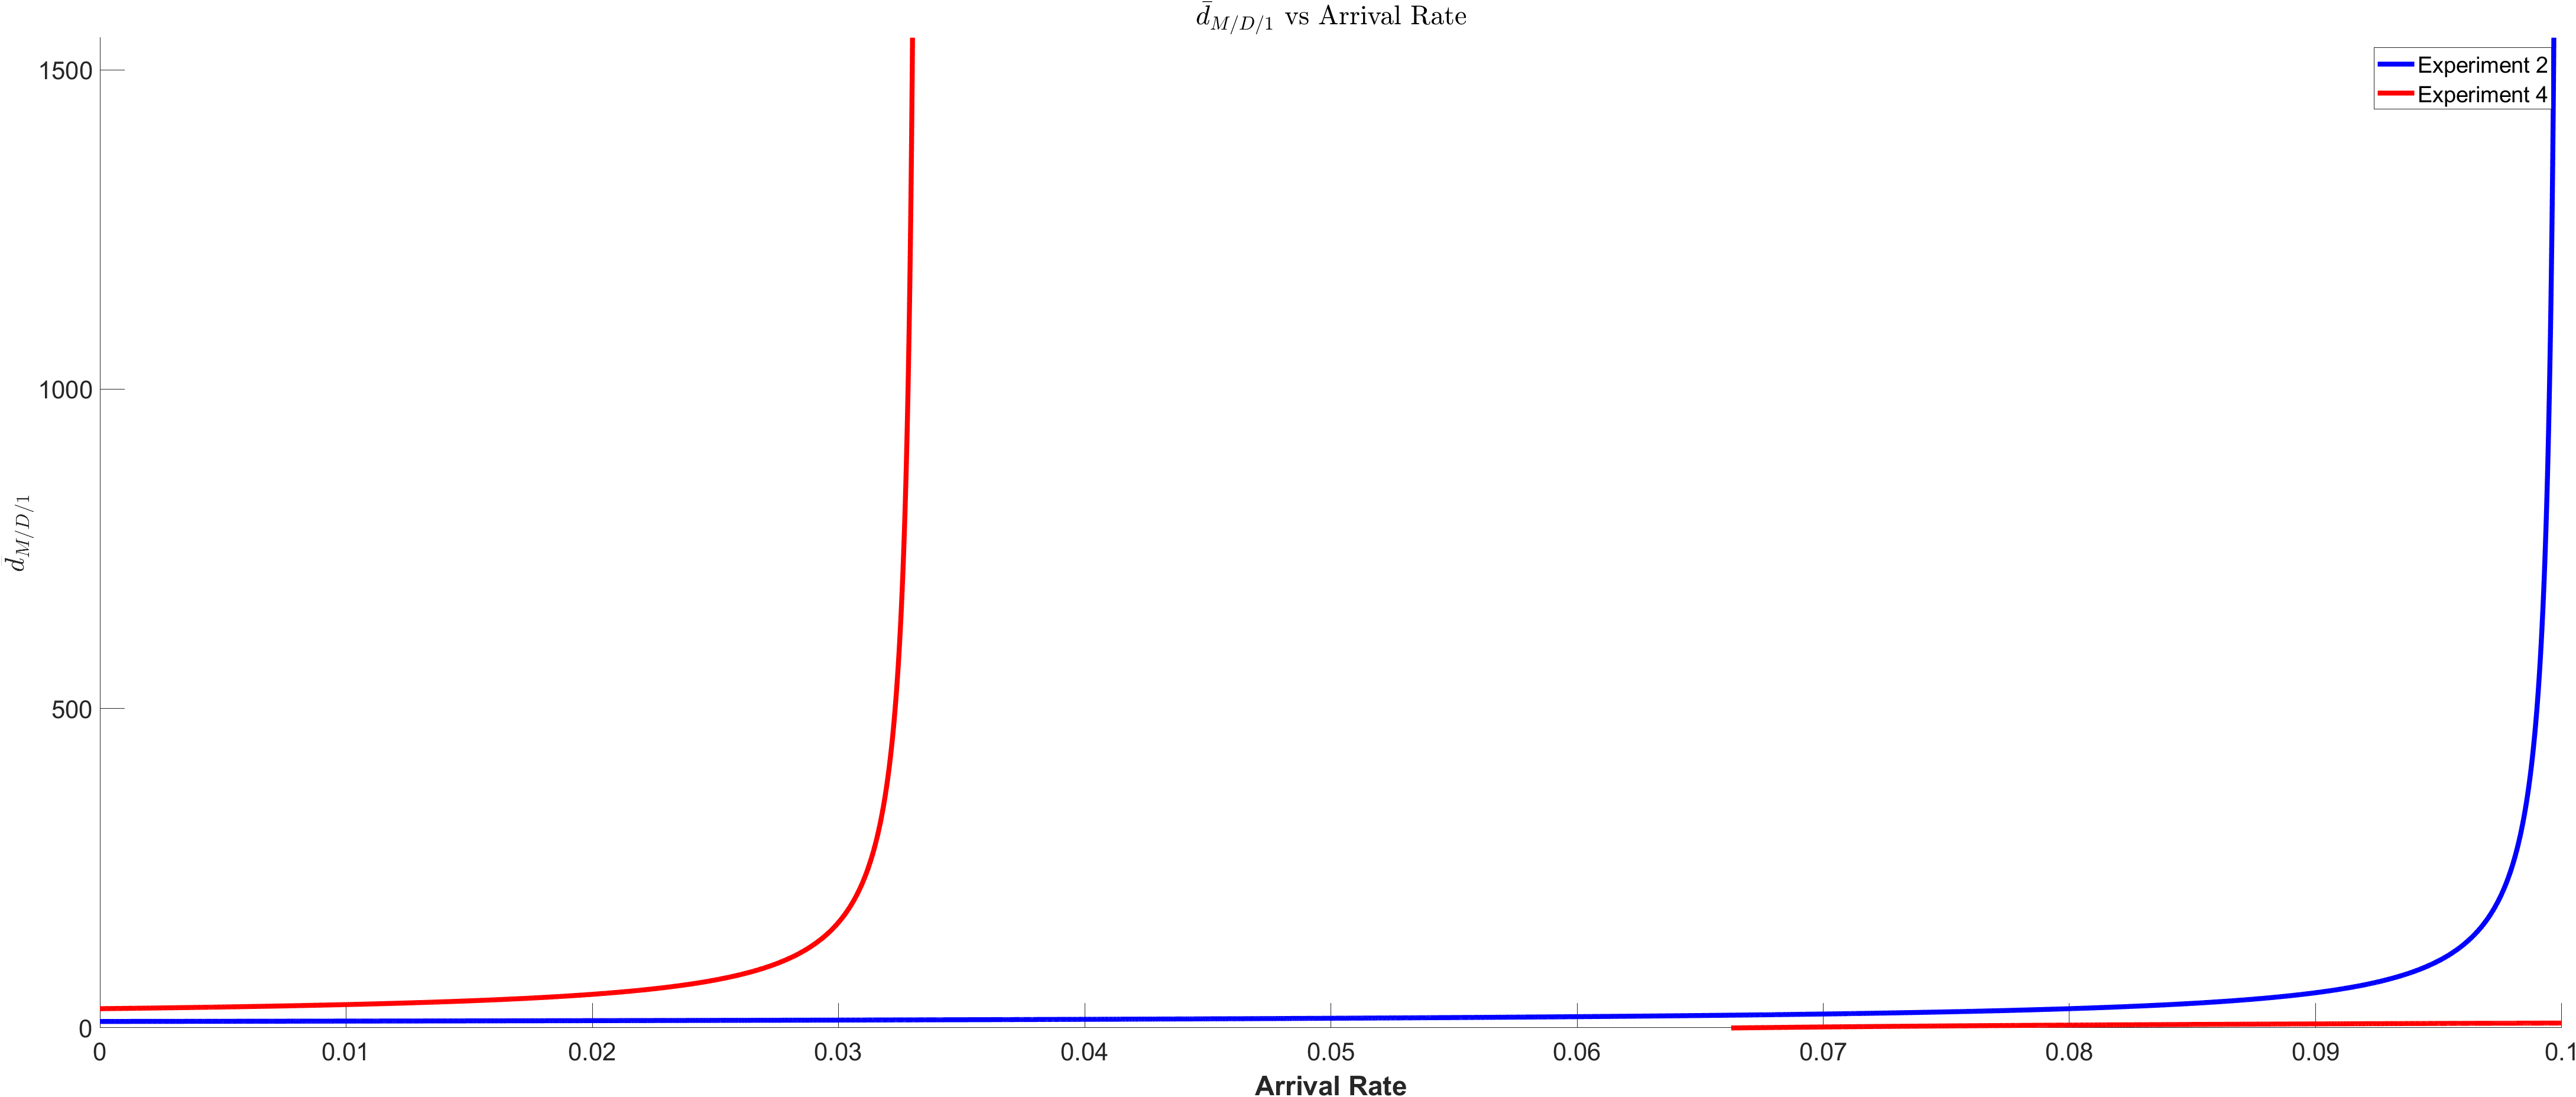
\includegraphics[width=\textwidth]{exp5.png}
    \caption{\label{fig:exp5}Mean Delay vs. Arrival Rate Plotted using Expression~\ref{eq:eq2}}
\end{figure}

\clearpage